\section{Wahrscheinlichkeitsmaße auf $\pmb{\R}$}
Kontinuierliche Ergebnisse lassen sich nicht mehr durch eine abzählbare Anzahl an Versuchsausgängen beschreiben.
Wahrscheinlichkeiten kann man dann nur noch \enquote{gutartigen Mengen} zuordnen, u.a.:
\begin{itemize}
	\item Intervalle sind gutartig
	\item Komplemente gutartiger Mengen sind gutartig
	\item Abzählbare Vereinigungen gutartiger Mengen sind gutartig
\end{itemize}
Bezeichne nun mit $\AG\subseteq\PG(\Omega)$ das System aller \enquote{gutartigen} Mengen.

\paragraph{Definition: $\pmb{\sigma}$-Algebra}
Sei $\Omega\neq\emptyset$ ein beliebiger Grundraum. Eine Menge $\AG\subseteq\PG(\Omega)$ heißt $\pmb{\sigma}$\textbf{-Algebra} auf $\Omega$, falls:
\begin{itemize}
	\item $\emptyset,\Omega\in\AG$
	\item $A\in\AG\implies A^{\mathsf{C}}\in\AG$
	\item $A_n\in\AG\;\forall n\in\N\implies\bigcup\limits_{n\in\N}A_n\in\AG$
\end{itemize}
$(\Omega,\AG)$ heißt dann \textbf{messbarer Raum}.
Die Mengen $A\in\AG$ heißen \textbf{Ereignisse}.

\paragraph{Definition: Borel-$\pmb{\sigma}$-Algebra}
Die \textbf{Borel-$\pmb{\sigma}$-Algebra} $\BG$ auf $\R$ beschreibt die kleinste $\sigma$-Algebra, welche alle Intervalle $(a,b]$ für beliebige $a,b\in\R$ enthält.

\paragraph{Definition: Wahrscheinlichkeitsmaß und Wahrscheinlichkeitsraum}
Sei $(\Omega,\AG)$ ein Messraum mit Grundraum $\Omega\neq\emptyset$ und $\sigma$-Algebra $\AG$.
Eine Abbildung $\PP:\AG\rightarrow[0,1]$ heißt Wahrscheinlichkeitsmaß auf $(\Omega,\AG)$, falls
\begin{itemize}
	\item $\PP(\Omega)=1$
	\item $A_n\in\AG,n\in\N$, disjunkt $\implies\PP(\bigcup\limits_{n\in\N}A_n)=\sum\limits_{n\in\N}\PP(A_n)$ \qquad($\sigma$-Additivität)
\end{itemize}
($\Omega,\AG\PP$) heißt dann \textbf{Wahrscheinlichkeitsraum}.

\newpage
\paragraph{Sätze und Definitionen für allgemeine Wahrscheinlichkeitsräume}
Folgende Sätze und Definitionen übertragen sich sinngemäß, wobei als Ereignisse jeweils nur Mengen aus $\AG$ betrachtet werden:
\begin{itemize}
	\item \hyperref[rules]{Rechenregeln für diskrete Wahrscheinlichkeitsmaße}
	\item \hyperref[conditioned]{Bedingte Wahrscheinlichkeiten}
	\item \hyperref[bayes]{Satz von der Totalen Wahrscheinlichkeit und von Bayes}
	\item \hyperref[independant]{Stochastische Unabhängigkeit von Ereignissen}
\end{itemize}
\underline{Unterschied}: Während diskrete Wahrscheinlichkeitsmaße $\PP$ vollständig durch die Zähldichte $f(\omega)\coloneqq\PP(\{\omega\}),\omega\in\Omega$ bestimmt sind, ist dies für allgemeine Wahrscheinlichkeitsmaße falsch!

\paragraph{Definition: Verteilungsfunktion}
Ist $\PP$ ein Wahrscheinlichkeitsmaß auf $(\R,\BG_{\R})$, so gilt für die durch
\begin{tightcenter}
	$F:\R\rightarrow[0,1], F(x)\coloneqq\PP((-\infty,x])$
\end{tightcenter}
definierte \textbf{Verteilungsfunktion} von $\PP$:
\begin{itemize}
	\item $F$ ist monoton steigend
	\item $F$ ist rechtsseitig stetig
	\item $F(\infty)\coloneqq\lim\limits_{x\rightarrow\infty}F(x)=1, \; F(-\infty)\coloneqq\lim\limits_{x\rightarrow-\infty}F(x)=0$
\end{itemize}
Ist umgekehrt $F:\R\rightarrow[0,1]$ eine Funktion, die obige Punkte erfüllt, so existiert genau ein Wahrscheinlichkeitsmaß auf $(\R,\BG_{\R})$, das $F$ als Verteilungsfunktion besitzt.
Für ein diskretes Wahrscheinlichkeitsmaß $\PP$ ist die Verteilungsfunktion eine Treppenfunktion.

\paragraph{Definition: Dichten}
Sei $\PP$ ein Wahrscheinlichkeitsmaß auf $(\R,\BG_{\R})$. Existiert eine integrierbare Funktion $f:\R\rightarrow[0,\infty)$, sodass
\begin{tightcenter}
	$F(x)=\PP((-\infty,x])=\int_{-\infty}^{x}f(t)dt$ \qquad$\forall x\in\R$
\end{tightcenter}
so heißt $f$ Dichte von $\PP$ bzw. von der zugehörigen Verteilungsfunktion $F$.
Für $A\in\BG_{\R}$ gilt dann
\begin{tightcenter}
	$\PP(A)=\int_{\R}f(x)\cdot\mathds{1}_A(x)dx\eqqcolon\int_{A}f(x)dx$
\end{tightcenter}
Umgekehrt ist jede integrierbare Funktion $f:\R\rightarrow[0,\infty)$ mit $\int_{-\infty}^{\infty}f(t)dt=1$ Dichte eines Wahrscheinlichkeitsmaßes auf  $(\R,\BG_{\R})$, das durch obiges $F$ eindeutig festgelegt ist.
Falls eine Dichte existiert, ist $F$ stetig.

Achtung: Dichten dürfen nicht mit Zähldichten verwechselt werden!

\paragraph{Definition: Gleichverteilung}
Für $-\infty<a<b<\infty$ heißt das Wahrscheinlichkeitsmaß auf $(\R,\BG_{\R})$ zur Dichte $f\coloneqq\frac{1}{b-a}\mathds{1}_{(a,b]}$ \textbf{Gleichverteilung} $U_{(a,b]}$ auf $(a,b]$ und für $a\leq c<d\leq b$ gilt:\\ $U_{(a,b]}((c,d])=\frac{d-c}{b-a}$.

\paragraph{Definition: Exponentialverteilung}
Die \textbf{Exponentialverteilung} $Exp_\lambda$ mit Parameter $\lambda>0$ ist gegeben durch die Dichte
\begin{tightcenter}
	$f_\lambda(x)\coloneqq\frac{1}{\lambda}e^{-x/\lambda}\cdot\mathds{1}_{[0,\infty)}(x)$, \qquad$x\in\R$
\end{tightcenter}
Die Verteilungsfunktion ist gegeben durch $F_\lambda(x)=1-e^{-x/\lambda}$, \qquad$\forall x\geq 0$\\ und $F_\lambda(x)=0$ für alle $x<0$.

Exponentialverteilungen beschreiben Lebensdauern von Dingen, die nicht altern, d.h. die Wahrscheinlichkeit noch $y$ Jahre zu überleben, gegeben dass bereits $x$ Jahre überlebt wurden, hängt nicht von $x$ ab.

\paragraph{Definition: Normalverteilung}
Die \textbf{Normalverteilung} $N_{(\mu,\sigma^2)}$ mit Parametern $\mu\in\R,\sigma>0$ ist gegeben durch die Dichte
\begin{tightcenter}
	$f(x)\coloneqq\cfrac{1}{\sqrt{2\pi\sigma^2}}\cdot exp(-\cfrac{(x-\mu)^2}{2\sigma^2})$, \qquad$x\in\R$
\end{tightcenter}
Die Verteilung $N_{(0,1)}$ wird \textbf{Standardnormalverteilung} genannt.
Die Verteilungsfunktion von $N_{(0,1)}$ bezeichnet man mit
\begin{tightcenter}
	$\Phi(x)=\int_{-\infty}^{x}\frac{1}{\sqrt{2\pi}}e^{-t^2/2}dt$
\end{tightcenter}
Aufgrund der Symmetrie der Standardnormalverteilung zur y-Achse, gilt\\ $\Phi(-x)=1-\Phi(x)$ für alle $x\in\R$.
Insbesondere ist $\Phi(0)=\frac{1}{2}$.

Für die Verteilungsfunktion der Normalverteilung $N_{(\mu,\sigma^2)}$ gilt
\begin{tightcenter}
	$F(x)=\Phi(\frac{x-\mu}{\sigma})$
\end{tightcenter}
Um Wahrscheinlichkeiten für eine beliebige Normalverteilung zu berechnen, genügt also die Verteilungsfunktion $\Phi$ der Standardnormalverteilung:\\\\
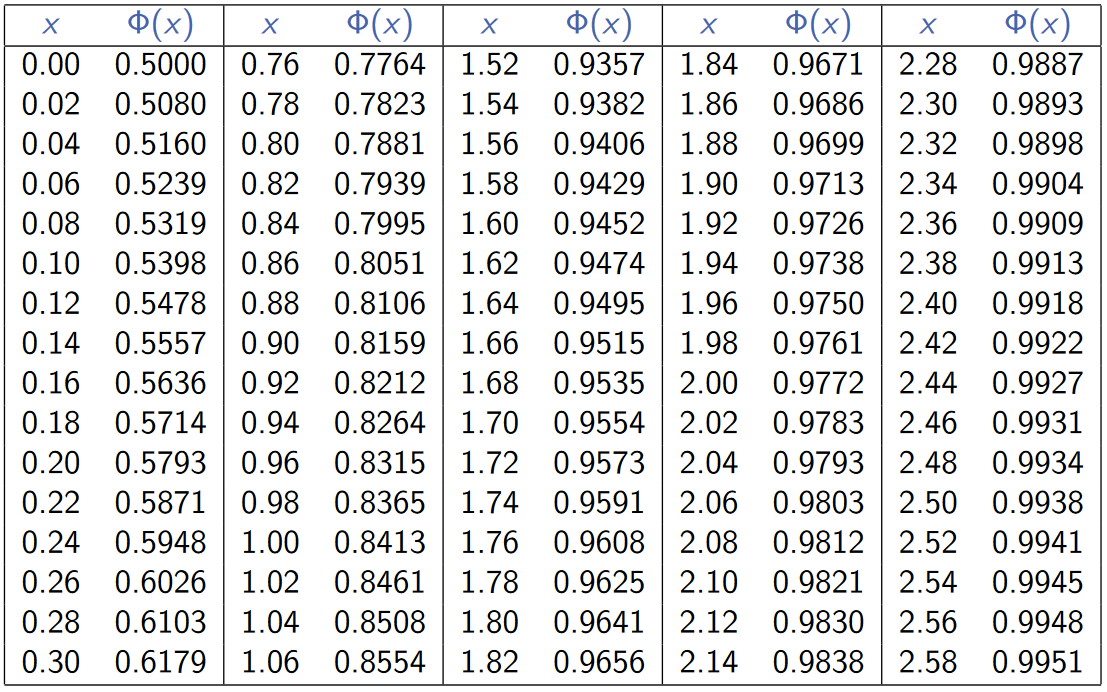
\includegraphics[width=\textwidth]{images/image2.png}

\paragraph{Definition: Zufallsvariable, Messbarkeit und Verteilung}
Eine Zufallsvariable $X$ ist nur noch definiert, wenn das Urbild von $X$ eine \enquote{gutartige} Menge ist.

Seien $(\Omega,\AG)$, $(S,\CG)$ messbare Räume und $X:\Omega\rightarrow S$ eine Abbildung.
$X$ heißt $S$-wertige \textbf{Zufallsvariable}, falls $X^{-1}(C)\in\AG$ für alle $C\in\CG$ ist.\\
Man schreibt $X:(\Omega,\AG)\rightarrow(S,\CG)$ und sagt, dass $X$ $(\AG,\CG)$\textbf{-messbar} ist.
Die sogenannte \textbf{Verteilung} von $X$ unter $\PP$ wird durch das Wahrscheinlichkeitsmaß
\begin{tightcenter}
	$\PP^X(C)\coloneqq\PP(X^{-1}(C))=\PP(X\in C)$, \qquad$C\in\CG$
\end{tightcenter}
auf $(S,\CG)$ definiert.

\newpage
\paragraph{Definition: Verteilungsfunktion und Dichte von Zufallsvariablen}
Sei $X:(\Omega,\AG)\rightarrow(S,\CG)$ eine $\R$-wertige Zufallsvariable auf dem Wahrscheinlichkeitsraum $(\Omega,\AG,\PP)$.
\begin{itemize}
	\item Die Verteilungsfunktion der Verteilung $\PP^X$ von $X$
	\begin{tightcenter}
		$F_X:\R\rightarrow[0,1],\; x\mapsto\PP^X((-\infty,x])=\PP(X\leq x)$
	\end{tightcenter}
	wird auch \textbf{Verteilungsfunktion} von $X$ genannt.
	\item $X$ heißt \textbf{stetige Zufallsvariable}, falls $F_X$ eine Dichte $f_X$ besitzt:
	\begin{tightcenter}
		$\PP(X\leq x)=\int_{-\infty}^{x}f_X(t)dt$ \qquad$\forall x\in\R$
	\end{tightcenter}
	$f_X$ heißt dann auch \textbf{Dichte} von $X$.
\end{itemize}